\documentclass[twoside,11pt]{homework}

\coursename{EECS E6892 Fall 2015} % DON'T CHANGE THIS

\studentname{Daniel Kronovet}       % YOUR NAME GOES HERE
\studentmail{dbk2123@columbia.edu}   % YOUR UNI GOES HERE
\homeworknumber{4}               % THE HOMEWORK NUMBER GOES HERE
\collaborators{mkt2126, jma2215}             % THE UNI'S OF STUDENTS YOU DISCUSSED WITH

\begin{document}
\maketitle

\section*{Problem 1}

\subsection*{Part A}

I did this it was fun.

\subsection*{Part B}

K = 2

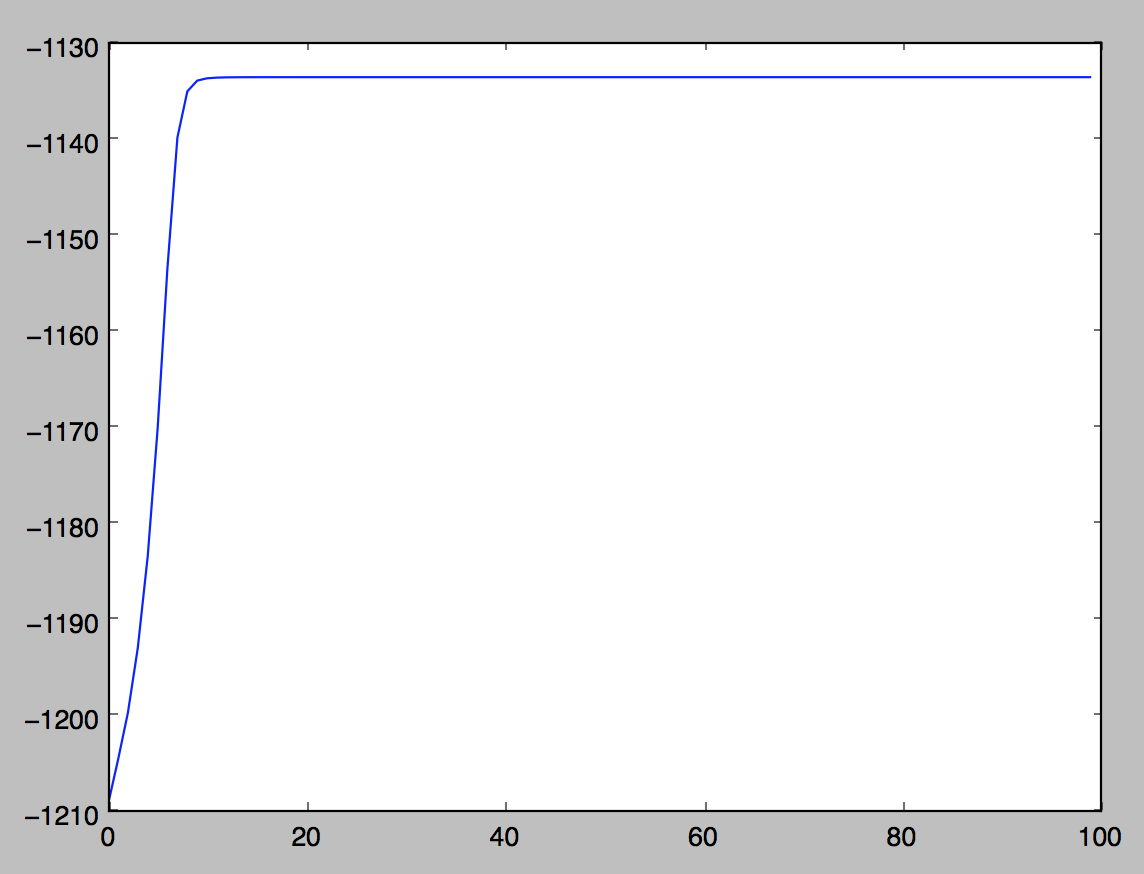
\includegraphics[scale=.5]{images/em_2_obj.png}

K = 4

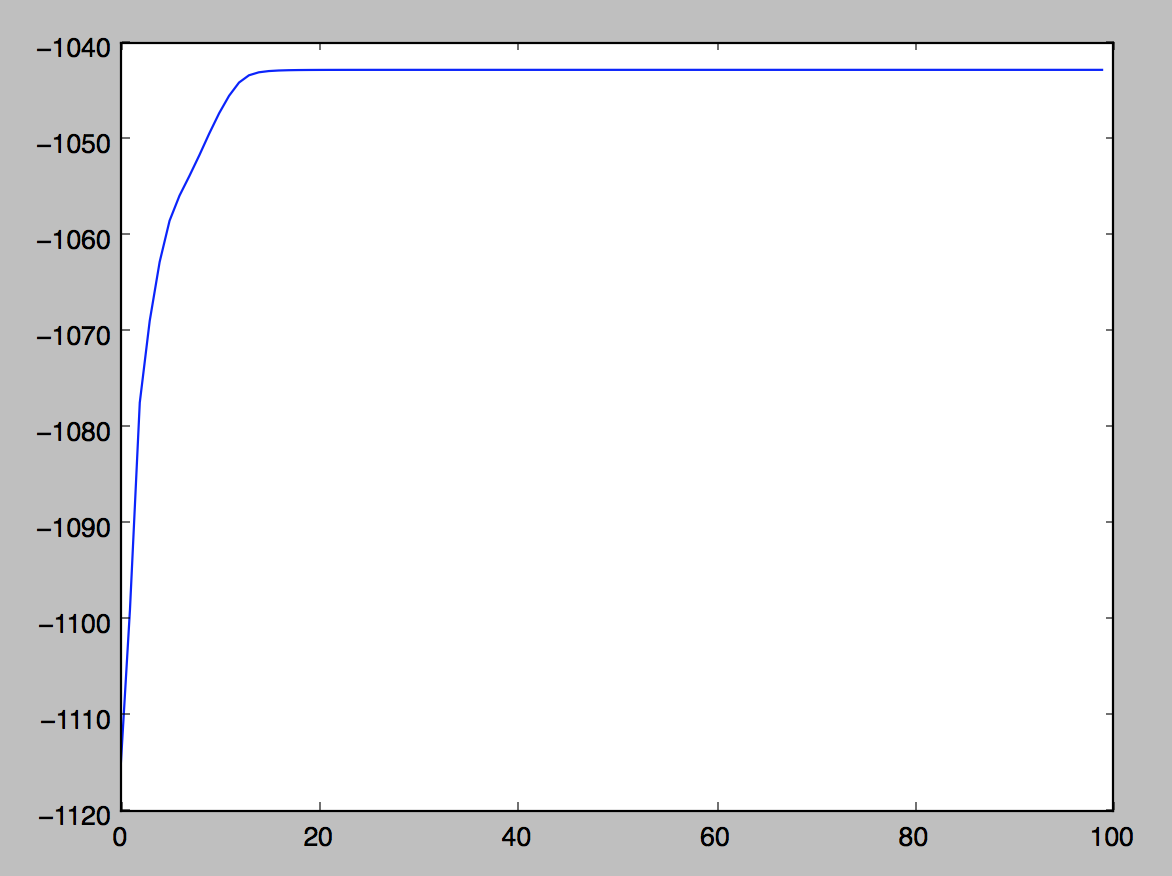
\includegraphics[scale=.5]{images/em_4_obj.png}

K = 8

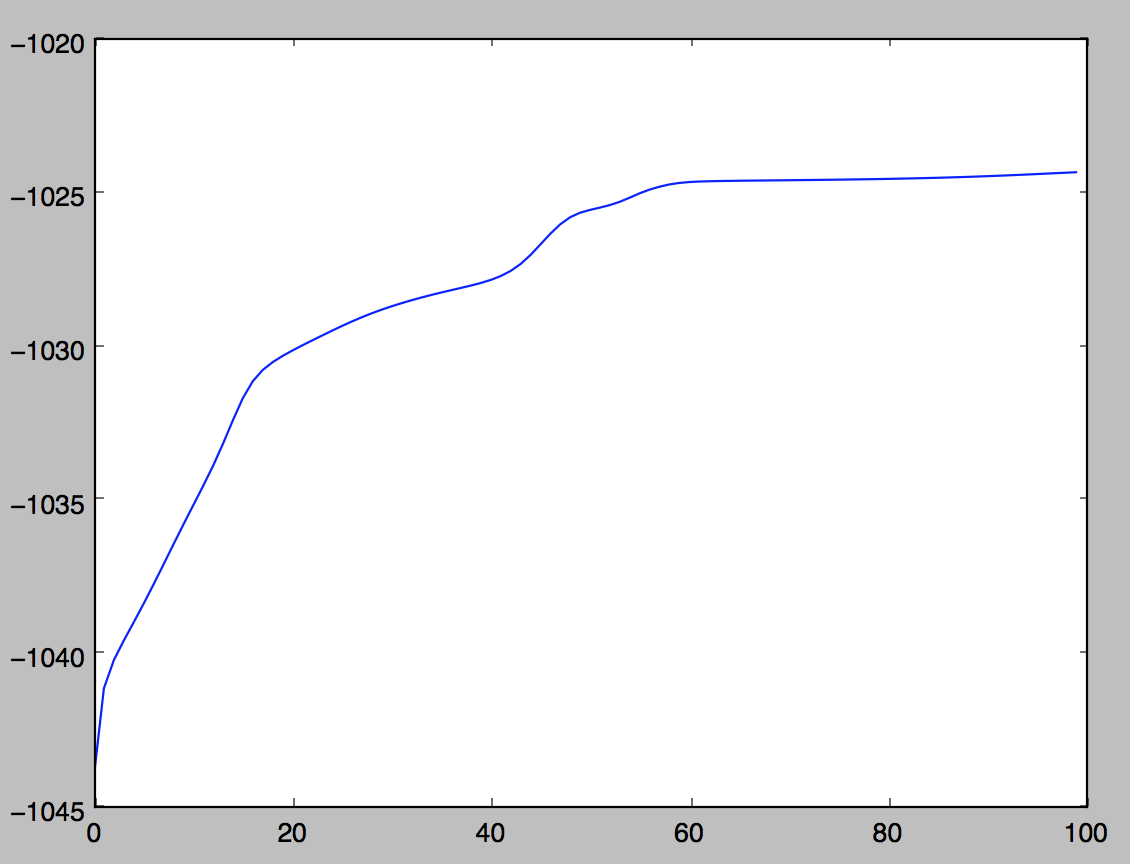
\includegraphics[scale=.5]{images/em_8_obj.png}

K = 10

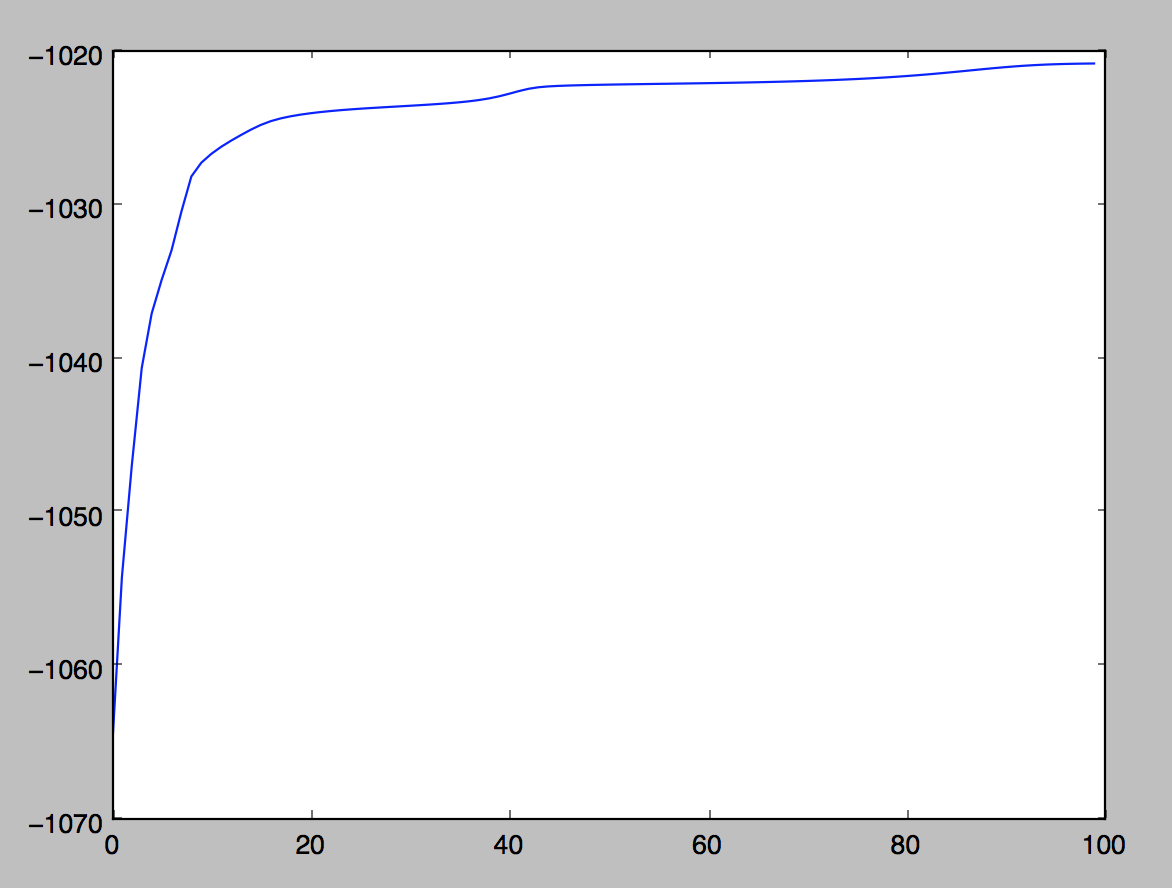
\includegraphics[scale=.5]{images/em_10_obj.png}

I notice that as K increases, the objective function converges more slowly, but converges to a higher overall likelihood. This makes sense as the algorithm is fitting a larger number of points; having more points minimizes the distance between any point and its cluster, increasing likelihood.

\subsection*{Part C}

K = 2

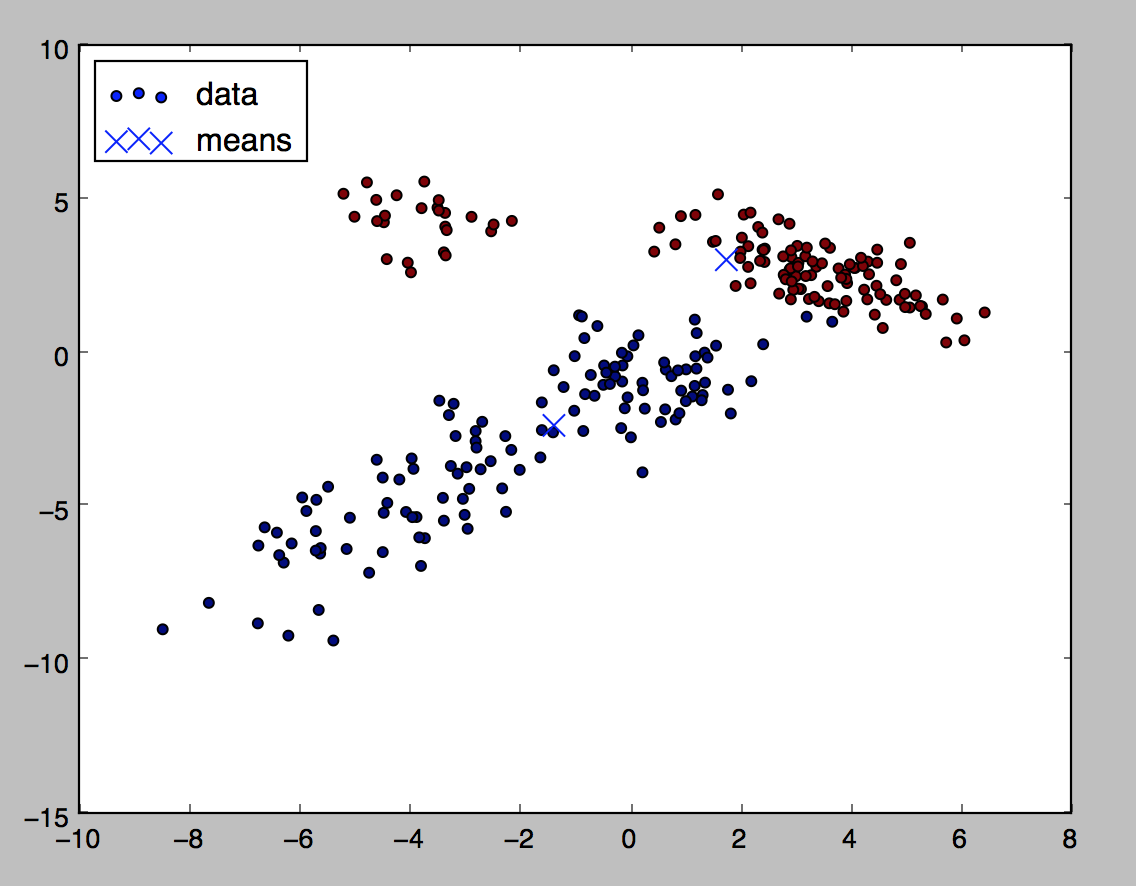
\includegraphics[scale=.5]{images/em_2_plot.png}

K = 4

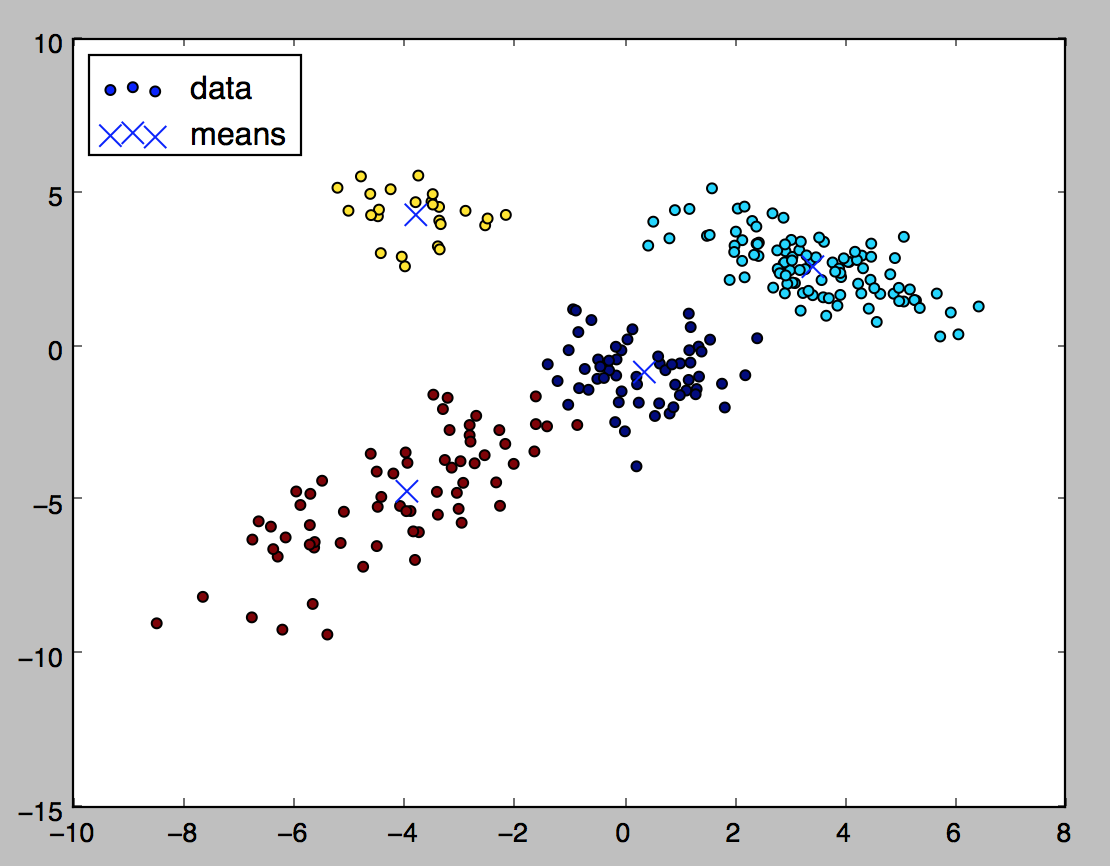
\includegraphics[scale=.5]{images/em_4_plot.png}

K = 8

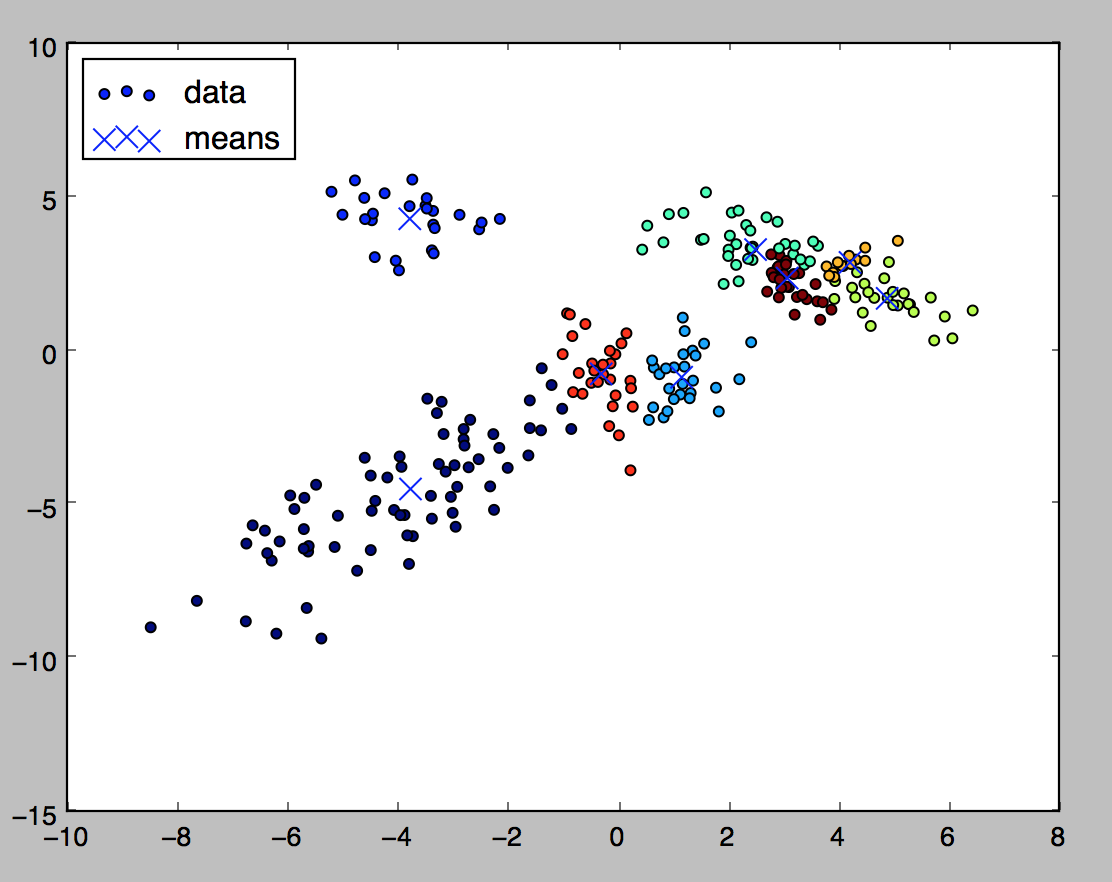
\includegraphics[scale=.5]{images/em_8_plot.png}

K = 10

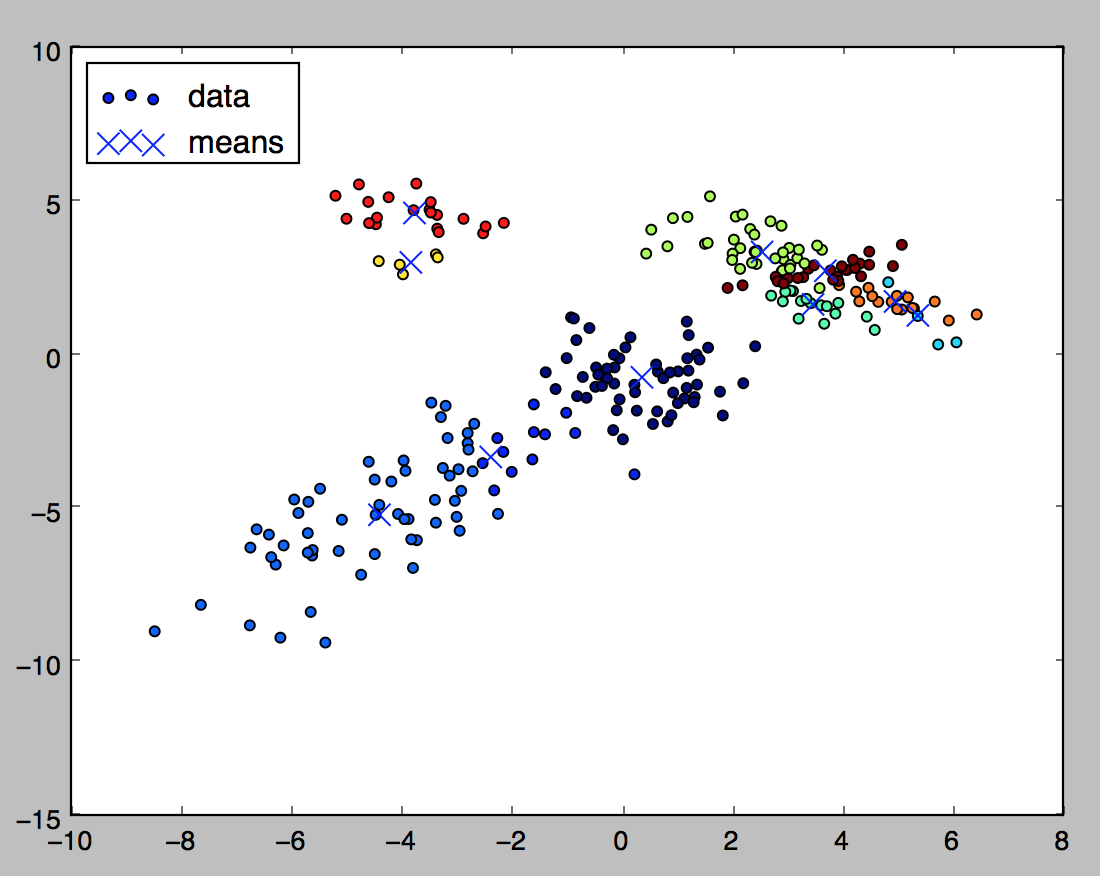
\includegraphics[scale=.5]{images/em_10_plot.png}

I noticed here that additional clusters tended to spread out over the points, minimizing overall error. When K=4, the clusters reflect what appears to be the true distribution. As K increases, the clusters spread out over the data, but reflect less the underlying structure.

\section*{Problem 2}

\subsection*{Part A}

I did this it was challenging.

\subsection*{Part B}

K = 2

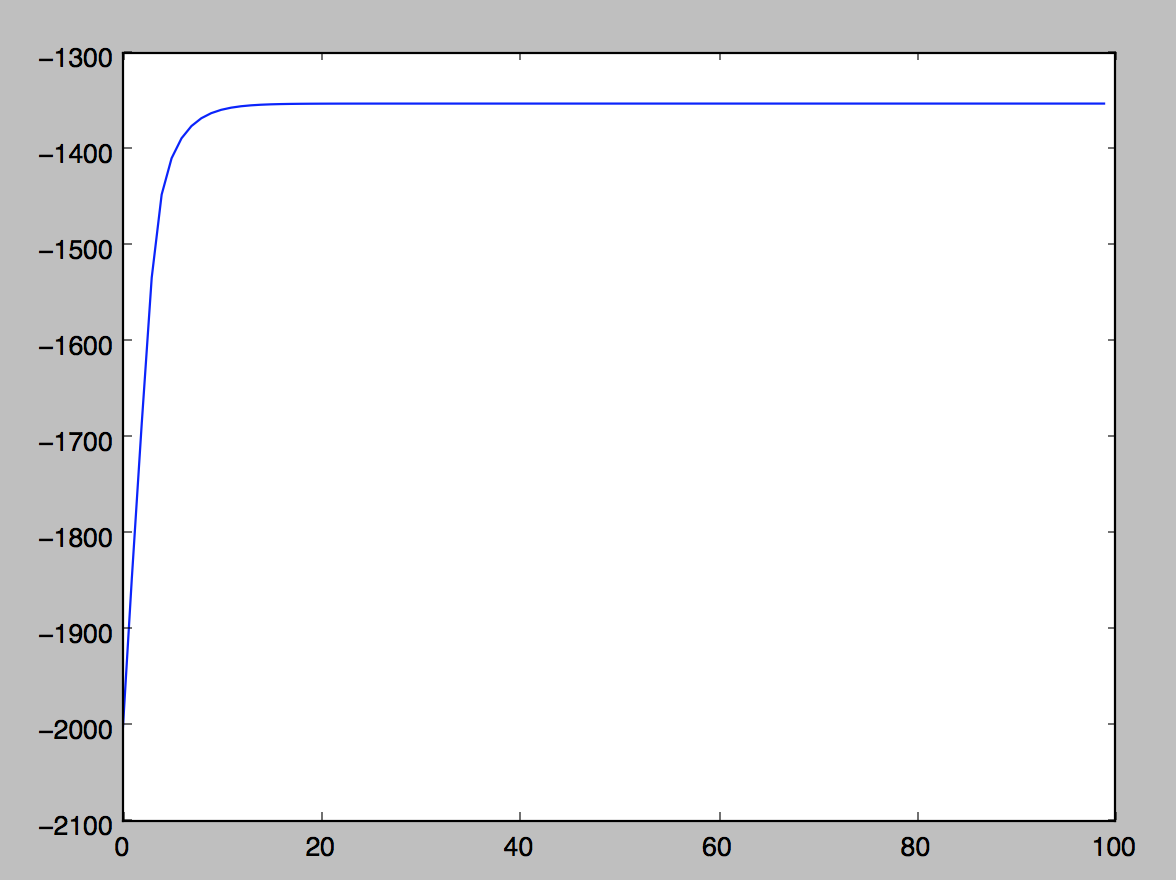
\includegraphics[scale=.5]{images/vi_2_obj.png}

K = 4

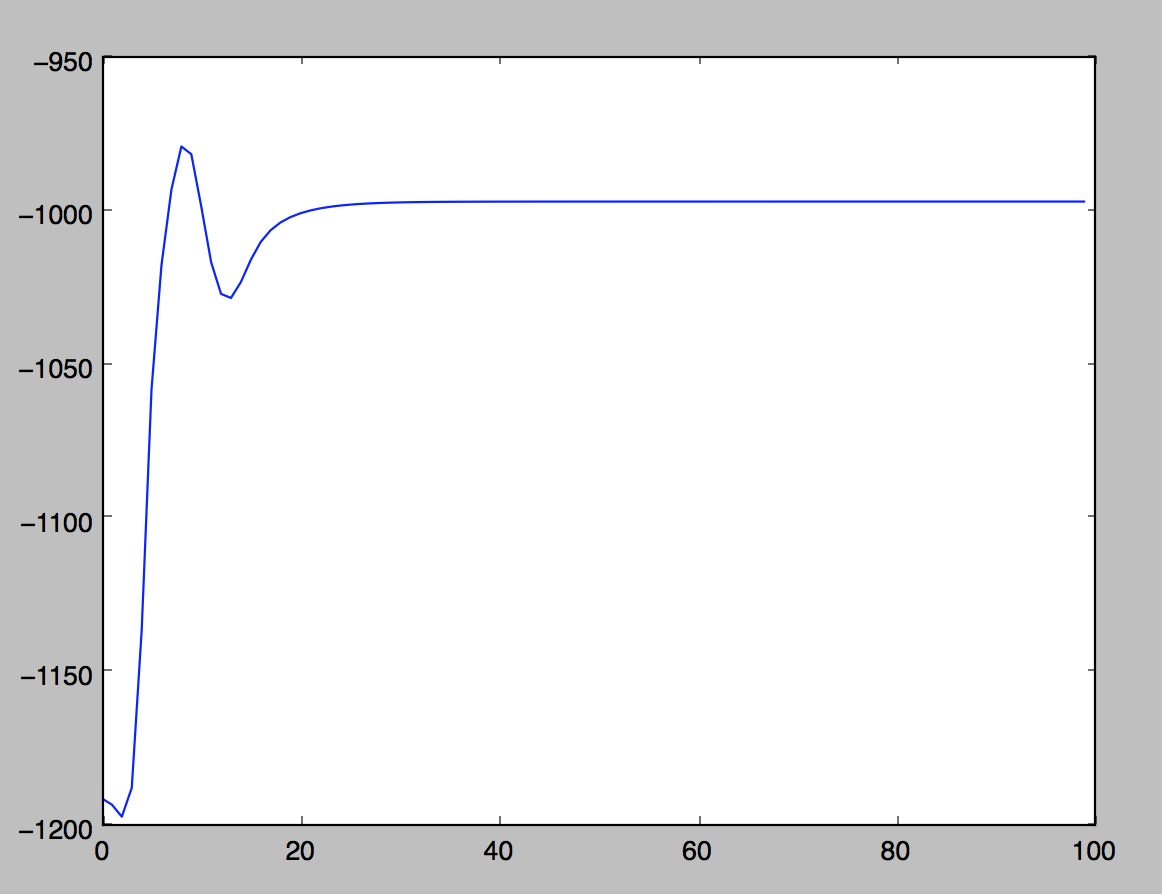
\includegraphics[scale=.5]{images/vi_4_obj.png}

K = 10

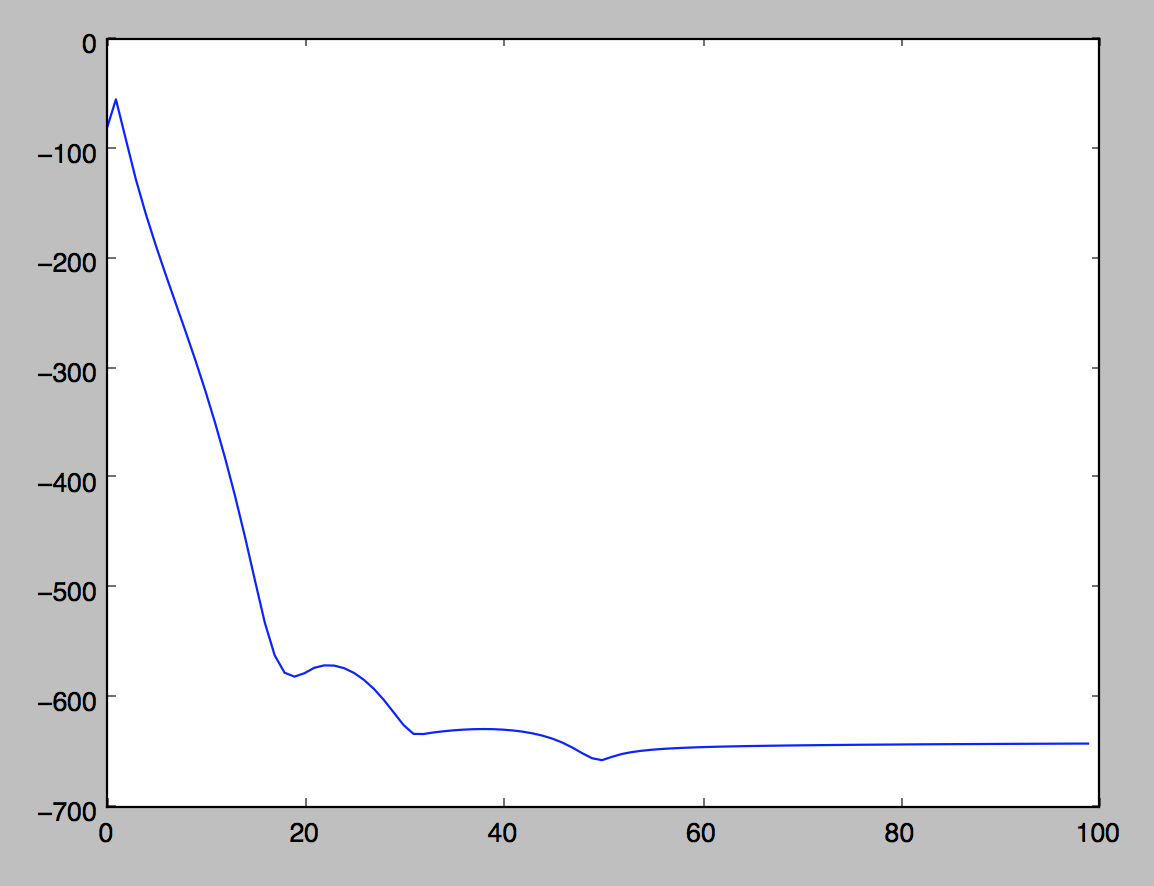
\includegraphics[scale=.5]{images/vi_10_obj.png}

K = 25

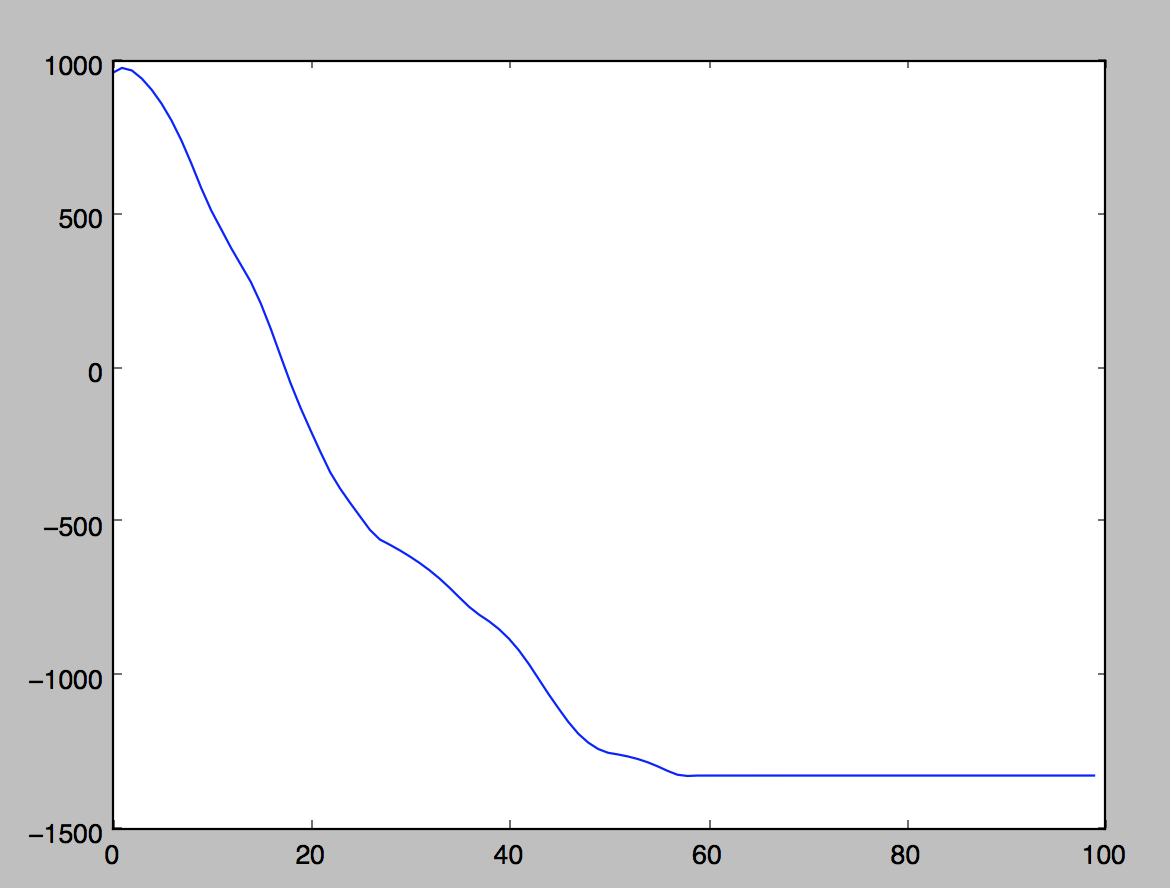
\includegraphics[scale=.5]{images/vi_25_obj.png}

I was unable to fully debug the VI objective function; it is not consistently monotonically increasing. My algorithm is performing well on data, however, so I believe the error is with the objective function itself.

\subsection*{Part C}

K = 2

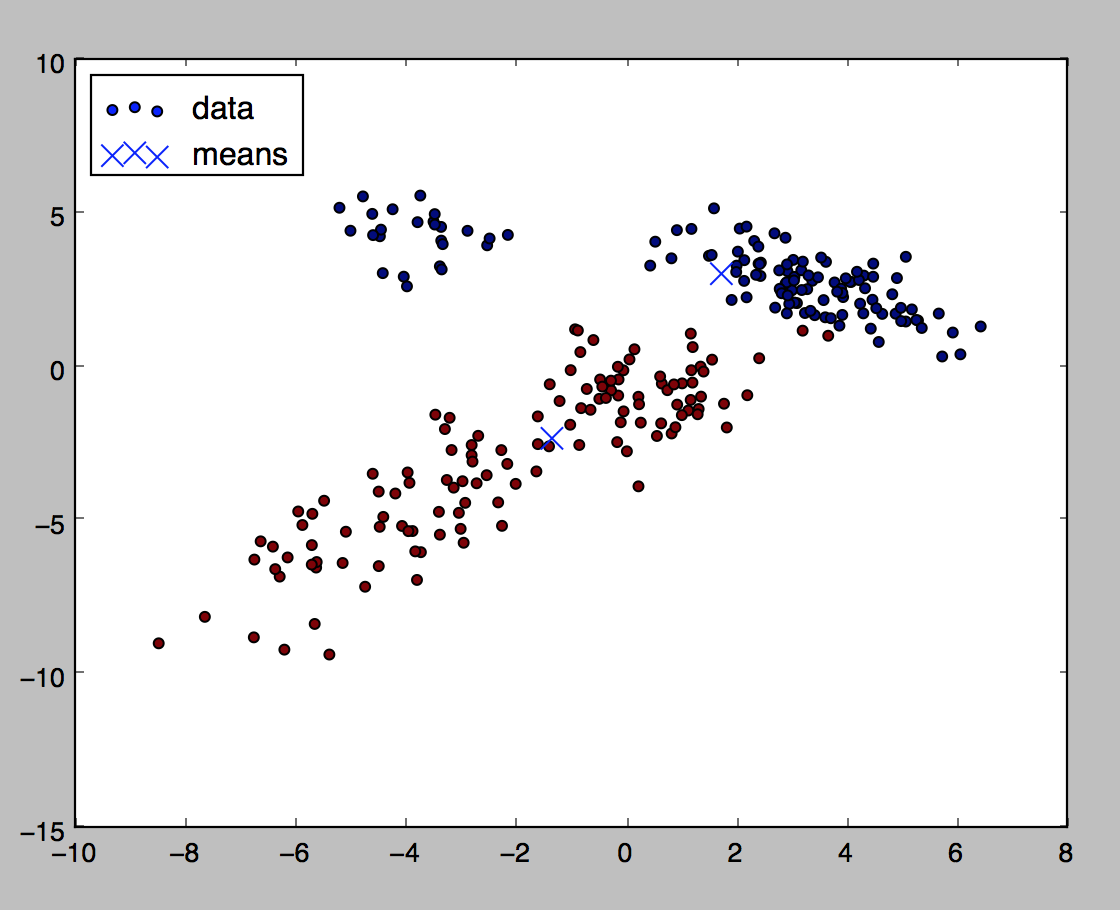
\includegraphics[scale=.5]{images/vi_2_plot.png}

K = 4

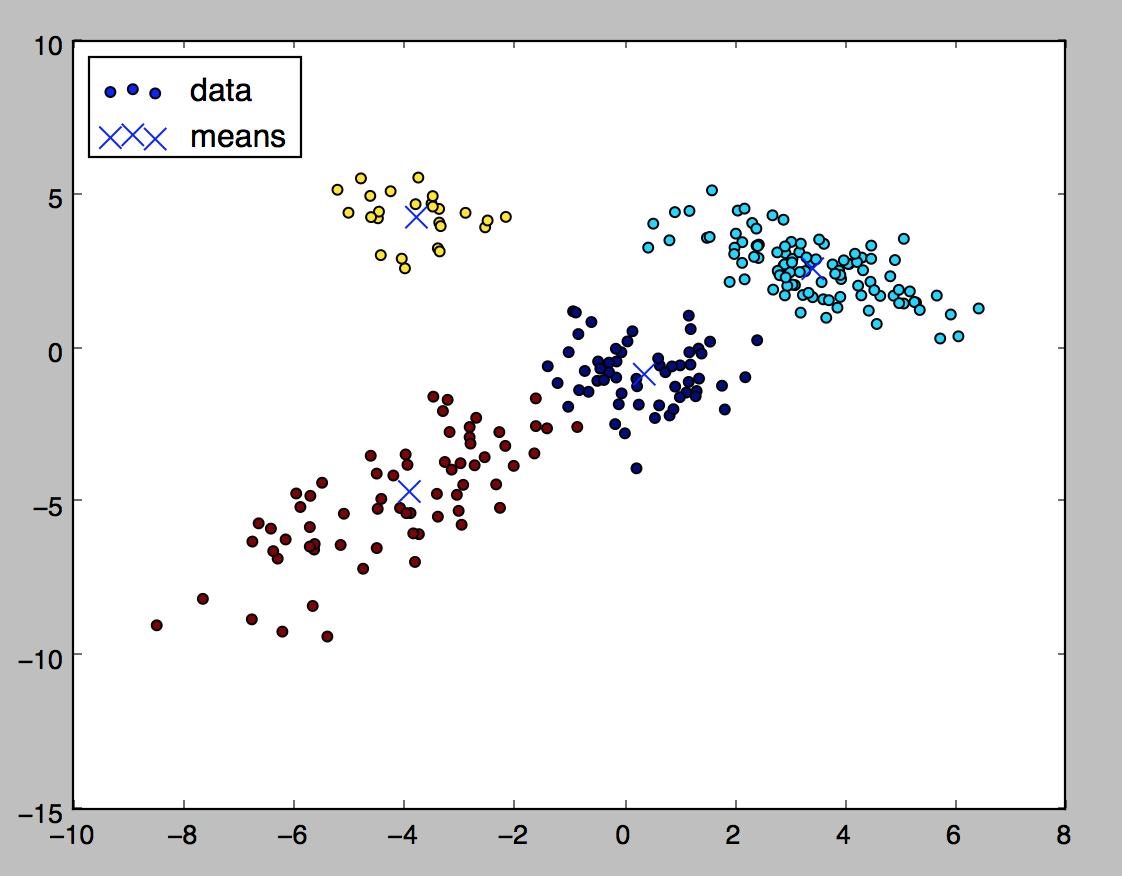
\includegraphics[scale=.5]{images/vi_4_plot.png}

K = 10

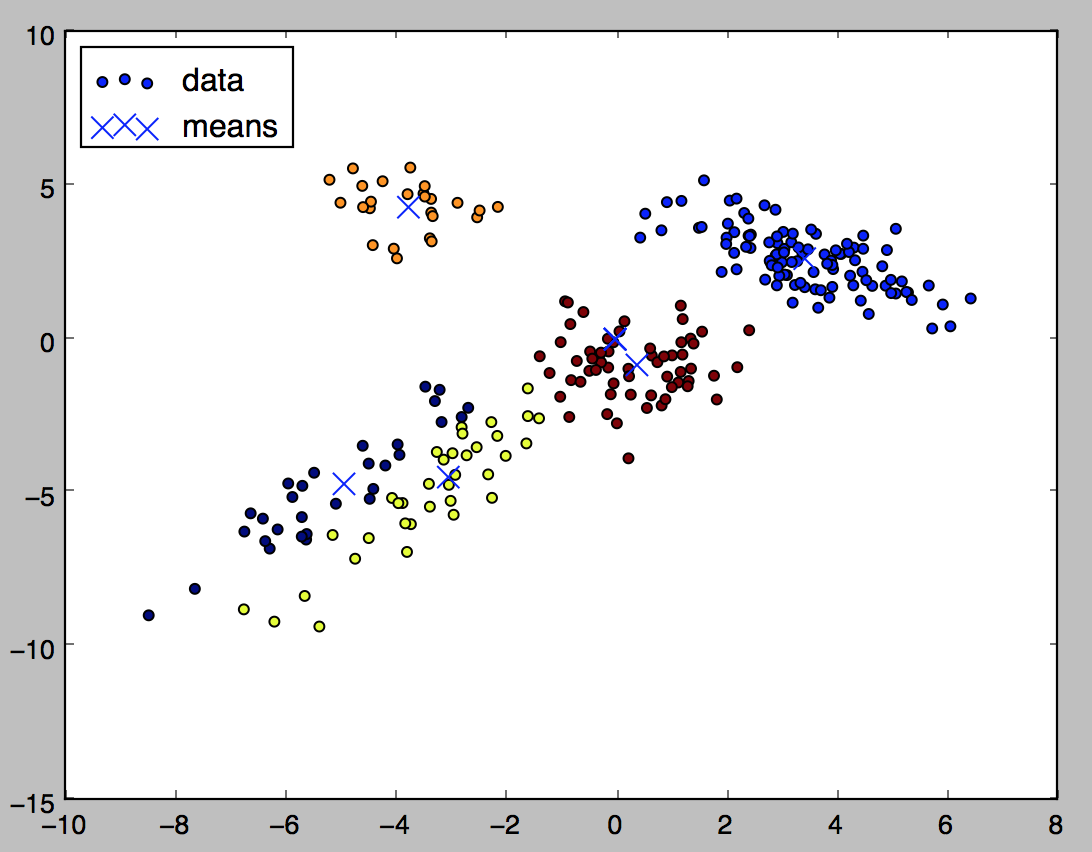
\includegraphics[scale=.5]{images/vi_10_plot.png}

K = 25

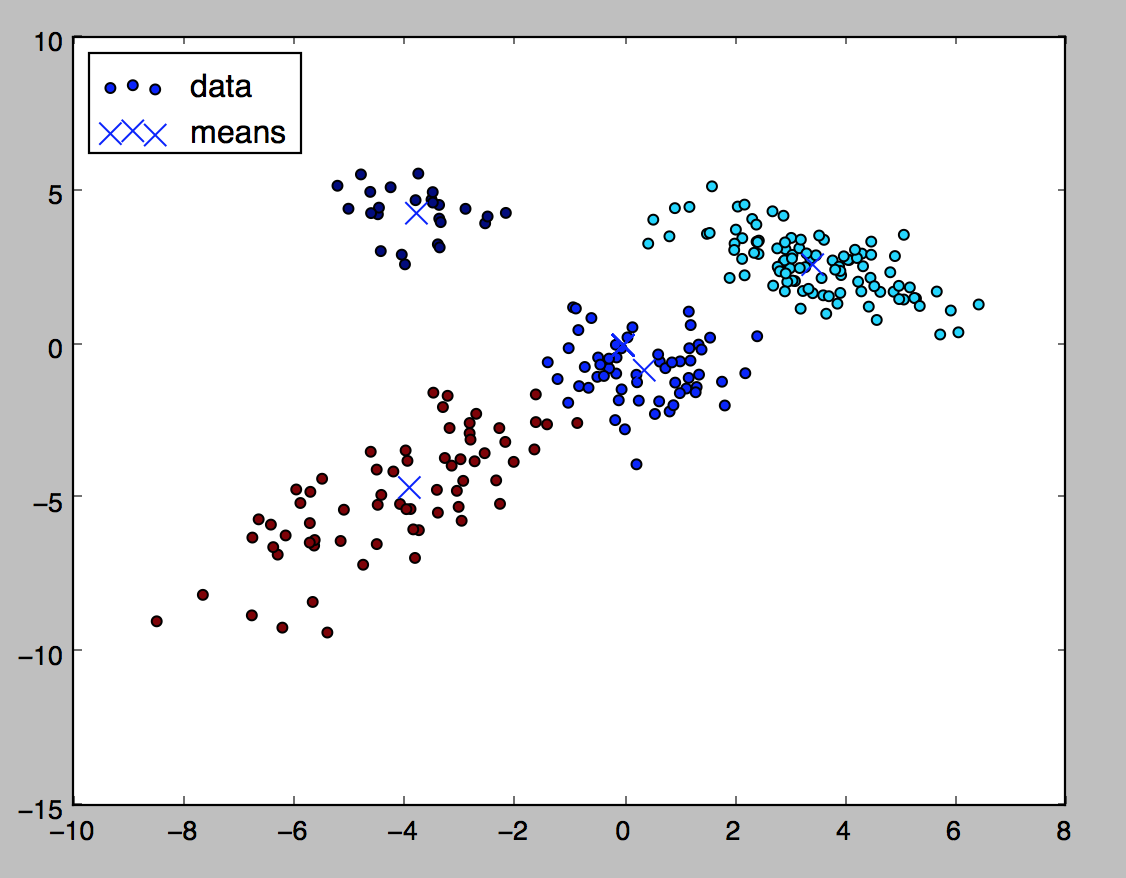
\includegraphics[scale=.5]{images/vi_25_plot.png}

I noticed that the VI algorithm will "learn" four clusters and place all of the density on those clusters; the density on the other points will go to zero, even though they are still being included in the algorithm.

\section*{Problem 3}

\subsection*{Part A}

I did this it was challenging.

\subsection*{Part B}

Points in top 6 clusters over 325 iterations (ended before 500 because the values were stable and it was past the HW submission deadline)

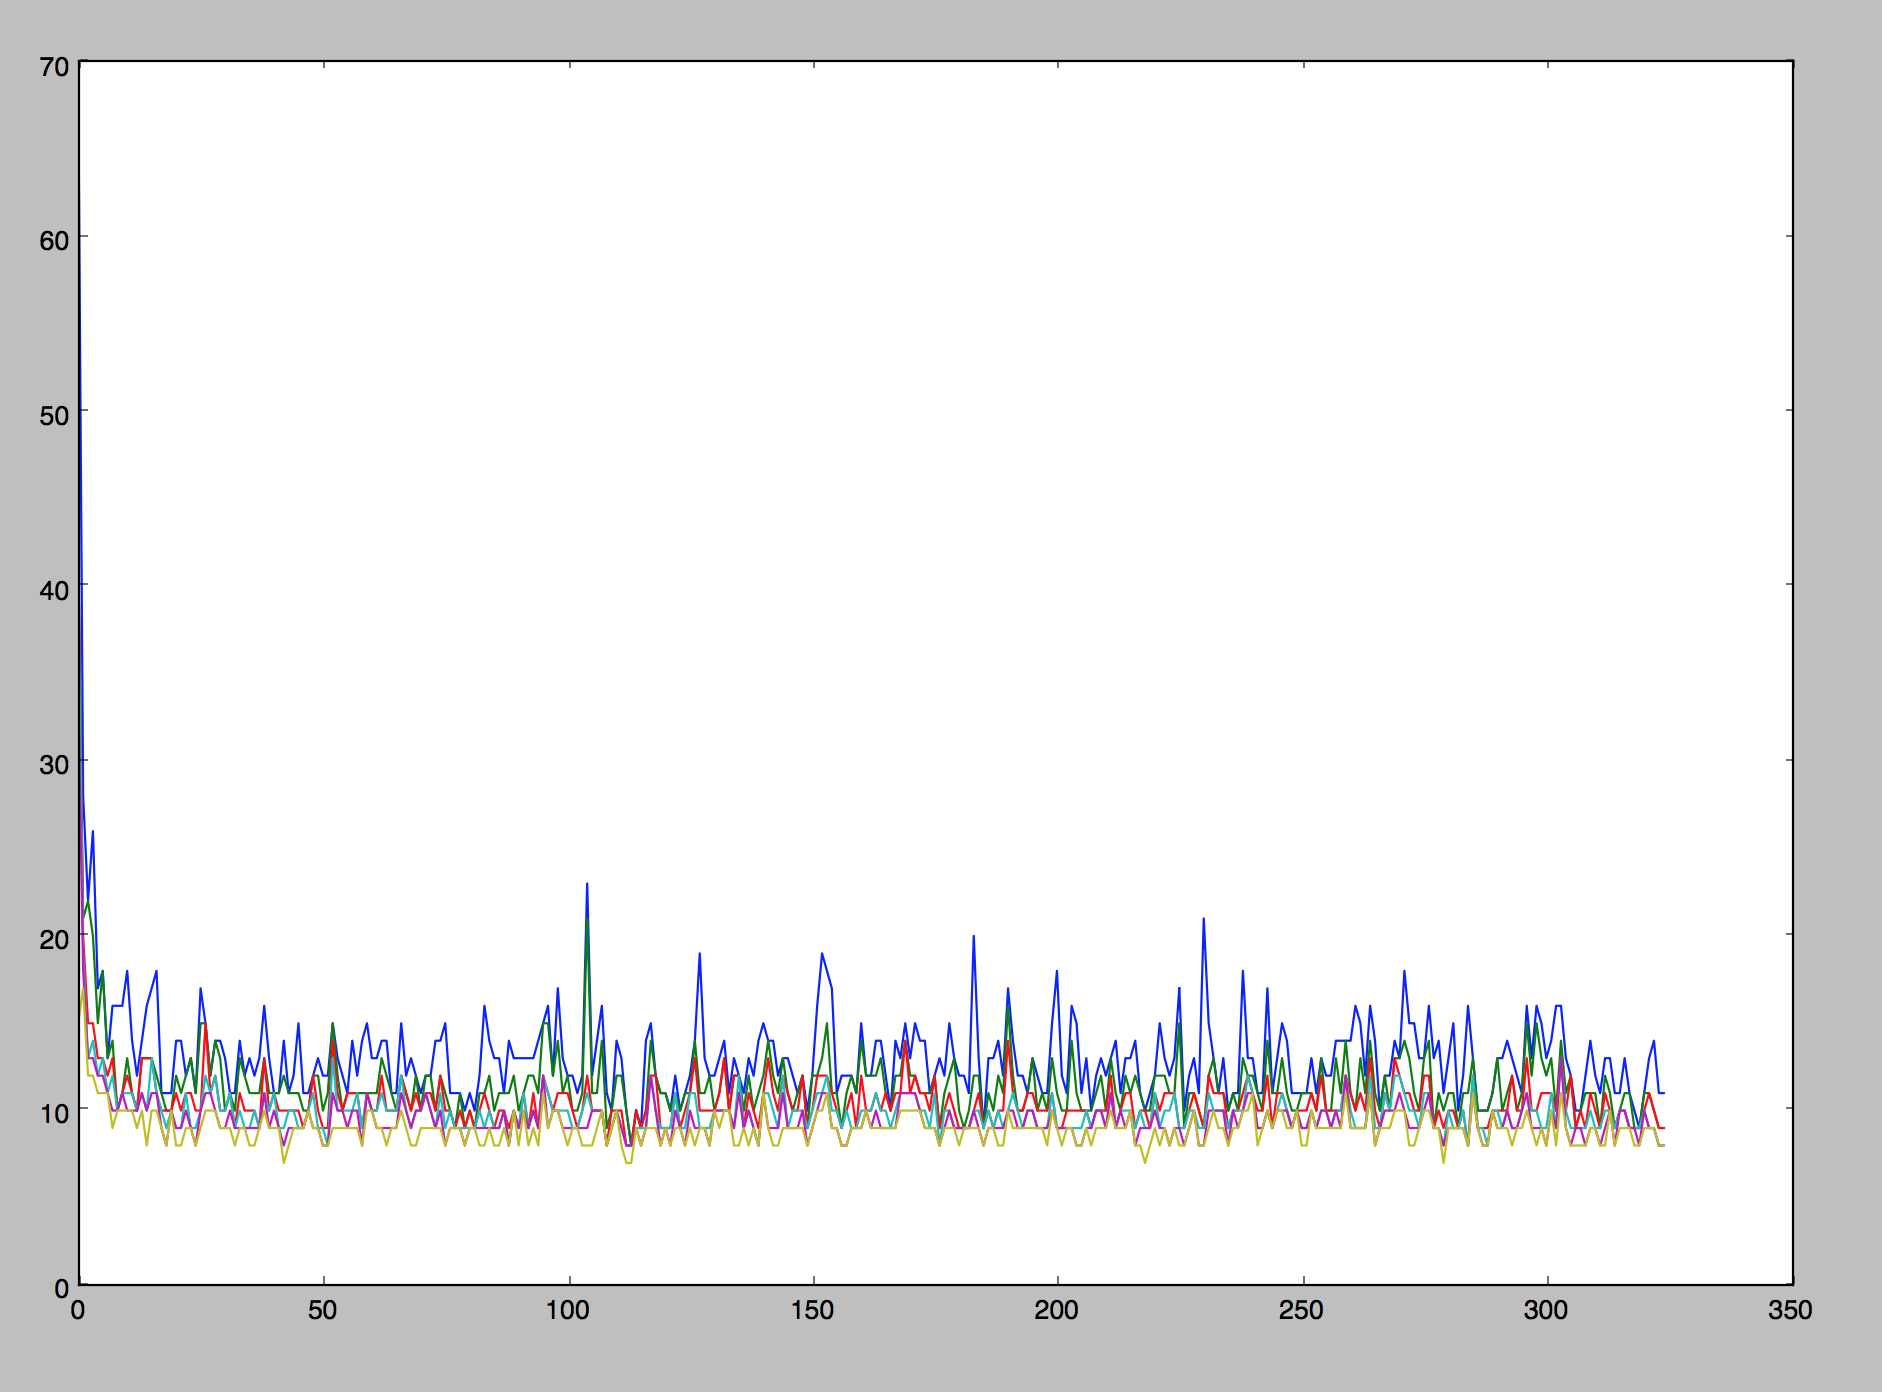
\includegraphics[scale=.5]{images/gibb_tops.png}

\subsection*{Part C}

Number of clusters over time -- stable in the ~50 cluster region.

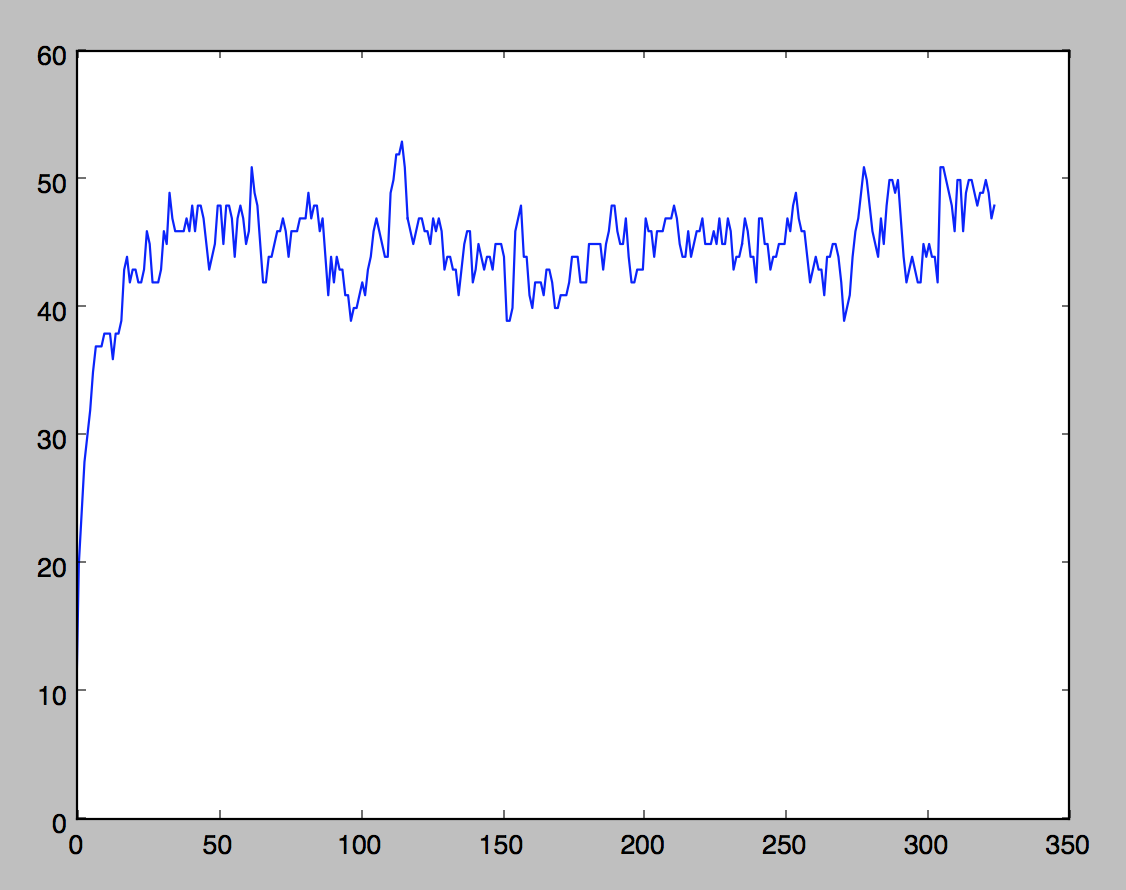
\includegraphics[scale=.5]{images/gibb_numc.png}

\end{document} 
